\documentclass{article}

\usepackage[%
    left=0.5in,%
    right=0.5in,%
    top=0.5in,%
    bottom=0.5in,%
]{geometry}%
\usepackage{minitoc}
\usepackage{multicol}
\usepackage{graphicx}
\usepackage{fixltx2e}
\usepackage{listings}
\usepackage{color}
\usepackage{hyperref}
    \hypersetup{ colorlinks = true, linkcolor = blue }
\usepackage{blindtext}
\definecolor{lightgray}{gray}{0.9}
\graphicspath{ {./} }

\newcommand{\inlinecode}[2]{\colorbox{lightgray}{\lstinline
[language=#1]$#2$}}
\newcommand{\worddef}[1]{\hyperref[sec:reference]{\textit{#1}}}

\definecolor{pblue}{rgb}{0.13,0.13,1}
\definecolor{pgreen}{rgb}{0,0.5,0}
\definecolor{pred}{rgb}{0.9,0,0}
\definecolor{pgrey}{rgb}{0.46,0.45,0.48}

\lstset{language=Java,
  showspaces=false,
  showtabs=false,
  breaklines=true,
  showstringspaces=false,
  breakatwhitespace=true,
  commentstyle=\color{pgreen},
  keywordstyle=\color{pblue},
  stringstyle=\color{pred},
  basicstyle=\ttfamily,
  moredelim=[il][\textcolor{pgrey}]{$ $},
  moredelim=[is][\textcolor{pgrey}]{\%\%}{\%\%}
}

\begin{document}

\tableofcontents

\newpage

\section{Thread	of	Execution}

\begin{flushleft}
Android applications use a \textbf{single thread model}. A single thread of execution called \textbf{main}. It is started when a process is created.
\begin{itemize}
  \item Handles and dispatches user interface events: drawing the interface, responding to interactions. E.g. onClick...()
  \item Handles activity lifecycle events: onCreate(), onDestroy…. For all components in an application
  \item HandlerThread
\end{itemize}
\end{flushleft}

\section{Looper and handler}

\begin{multicols}{2}

\begin{itemize}
  \item HandlerThread
  \begin{itemize}
    \item Extension of Thread with support for a Looper
  \end{itemize}
  \item Looper
  \begin{itemize}
    \item Each HandlerThread can have one Looper
    \item A Java thread dies when the run method returns
    \item Maintains a MessageQueue
    \item Looper.loop(): loops through the MessageQueue and processes waiting Messages
  \end{itemize}
  \item Message
  \begin{itemize}
    \item A	task	to	be	completed
    \item Might	contain	data,	reference	to	a	Runnable	object
  \end{itemize}
  \item Handler
  \begin{itemize}
    \item Attached to a Looper 
    \item Enqueues messages in the Looper MessageQueue
    \item Configurable delivery
    \item Handles messages from the MessageQueue
    \item Threadsafe
    \item  One Looper can have many Handlers associated with it
  \end{itemize}
\end{itemize}

\vfill\null

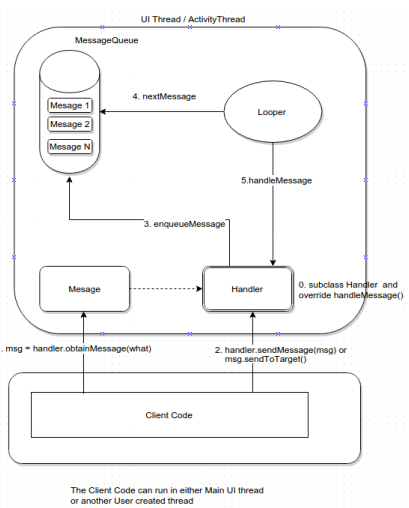
\includegraphics[scale=0.7]{Screenshot_2018-10-22_14-04-33.png}

\end{multicols}

\subsection{Splitting threads}
\begin{itemize}
\item Long (ish) running code that does not involve the UI
\begin{itemize}
  \item E.g. an image download 
  \item Occurs in a separate thread of execution
  \item Still tightly coupled to an activity
  \item Not allowed to do network communication in the UI thread
\end{itemize}
\item Instantaneous code that does involve the UI
\begin{itemize}
  \item E.g. drawing the image that has been downloaded
  \item posted to the UI thread responsible for a particular View to execute, logically parceled up as a Runnable object
  \item Risk of orphaned threads
\end{itemize}
\end{itemize}

\section{AsyncTask}
\begin{flushleft}
A convenience class for making complex asynchronous worker tasks easier. Worker / blocking tasks are executed in a background thread.
Can get data back using \textbf{results callback}, and it's executed in the UI thread. With each AsyncTask that is spun off, a thread is created and destroyed, which might be a performance issue. We can solve this by implementing implement a thread pool.
\end{flushleft}

\section{Services}
\begin{flushleft}
An	Application	Component	that
\begin{itemize}
  \item Has	no	UI
  \item Represents	a	desire	to	perform	a	longer-running	operation. I.e.	longer	than	a	single-activity	element	of	the	task
  \item Threads	are	associated	with	the	activity	that	started	them i.e.	could	be orphaned
\end{itemize}
Activities	are	loaded/unloaded	as	users	move	around	app, where as services	\textbf{remain	for	as	long	as	they	are	needed}.
Can expose	functionality	for	other	apps: one	service	\textbf{may	be	used	by	many	applications}, which allows to avoid	duplication	of	resources
\end{flushleft}


\subsection{What services are not}
\begin{itemize}
  \item Not a separate process
  \begin{itemize}
    \item Runs in the same process as the application in which it is declared (by default) 
  \end{itemize}
  \item Not a thread
  \begin{itemize}
    \item One thread per Application
    \item Handles events for all components
    \item If you need to do things in the background, start your own thread of execution
  \end{itemize}
\end{itemize}

\subsection{Uses of Services}
\begin{itemize}
  \item MP3	Playback: Want to play audio while the user is doing other things
  \item Network Access: long download, sending email, polling email server for new mail.
  \item Anything	that	you	don’t	want	to	interrupt	the	user	experience	for
\end{itemize}

\subsection{Creating a Service}
Services	are	designed	to	support	communication	with
\begin{itemize}
  \item Local	Activities	(in	the	same	process). For example: within	VM
  \item Remote	Activities	(in	a	different	process). For example IPC
  \item Multiple	components
  \begin{itemize}
    \item System services	underpin	much	of	Android	core	OS,	but	wrapped	with	various	APIs
  \end{itemize}
\end{itemize}
Services	are	components,	similar	to	an	Activities
\begin{itemize}
  \item Register	the	service	in	the	\textbf{manifest}
  \item Create	a	subclass	of	android.app.Service
  \item Handle	the	relevant	\textbf{lifecycle	methods}
\end{itemize}

\subsection{Service lifecycle}
There are two ways of spawning a service:\\
\textbf{Started	(loosely	coupled)}
\begin{itemize}
  \item Send an Intent to explicitly start the service with startService()
  \item c.f. Messages, starting Activities
  \item Will run / exist in the background indefinitely / until kills itself (Does not “return” results). For example: C.f email checking.
  \item Explicitly stop the service with stopService()
  \item User starts and stops it
\end{itemize}
\textbf{Bound	(tightly	coupled)}
\begin{itemize}
  \item Bind to a service using bindService()
  \item Will run while any Activities are bound to it
  \item Actively using it
  \item Provides an interface (programmatic) for Activities to communicate with the Service
  \item Operating system starts and stops it
\end{itemize}

\begin{flushleft}
In both cases, if the service is not running it \textbf{will be created}. Note both are \textbf{the same service}. Different responsibilities for the lifecycle (If I start it, I have to stop it. If OS starts it, OS stops it when it decides to)
\end{flushleft}

\begin{center}
  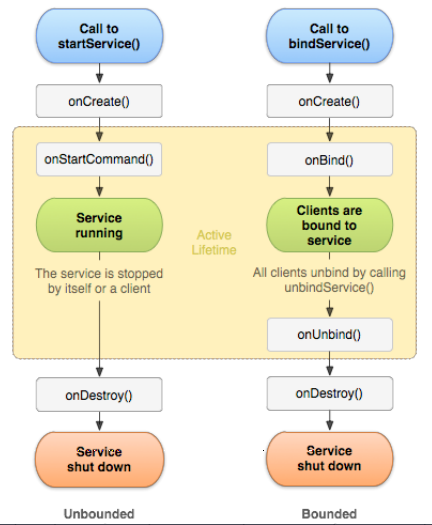
\includegraphics[scale=0.8]{threads.png}
\end{center}

By nature, services are singleton objects (there can be only one). Service used by \textbf{many clients}. The Service sub-class object is instantiated if necessary
\begin{itemize}
  \item \texttt{onCreate()} is called
  \item Either \texttt{onStartCommand} or \texttt{onBind} will be called depending on how the service has been "called"
  \item \texttt{onCreate} / \texttt{onStart} / \texttt{onBind} are called in the \textbf{context of the main UI thread}. It now must spawn a worker thread to do any significant work
  \item Something calls \texttt{stopService()}, (could be the OS or user again)
  \item \texttt{onDestroy} can now be used to save work.
\end{itemize}

\subsection{Implementing a service}

\begin{flushleft}
Generic	started	service
\begin{itemize}
  \item Runs persistently (Or stops itself when all work is done)
  \item Receives messages asking for more work to be done (Delivered via onStartCommand)
\end{itemize}
IntentService
\begin{itemize}
  \item A simple, unbound service.
  \begin{itemize}
    \item It assumes we don’t have multiple requests that need to be handled concurrently.
    \item Creates a queue of work to be done.
    \item HandlerThread, Looper, Handler again. 
  \end{itemize}
  \item Handles one intent at a time to onHandleIntent()
  \begin{itemize}
    \item Intents delivered via onStartCommand added to a queue
    \item Stops the service after all start requests have been handled
    \item I.e. sending emails “fire and forget”
  \end{itemize}
\end{itemize}
\end{flushleft}

\subsection{Terminating services}
\begin{flushleft}
A Service runs in the background indefinitely, even if the component that started it is destroyed.
\begin{itemize}
  \item Termination of a service
  \begin{itemize}
    \item Self-termination (calling stopSelf())
    \item stopService() via an Intent 
    \item System termination (i.e. memory shortage – Last recently used again)
  \end{itemize}
  \item Avoiding termination as a foreground service
  \begin{itemize}
    \item This is something the user should really know about or is aware of
    \item Active in the Status Bar / shows a Notification 
    \item Is treated as important as a foregrounded Activity
    \item startForeground(…)
  \end{itemize}
\end{itemize}
Because services run indefinitely, we can use onStartCommand where return value determines how the service should be continued if it is destroyed.
\begin{itemize}
  \item \verb|START_NOT_STICKY|
  \begin{itemize}
    \item After onStartCommand returns, do not recreate the service unless there are intents to deliver
  \end{itemize}
  \item \verb|START_STICKY|
  \begin{itemize}
    \item Recreate the service and call onStartCommand again, but do not redeliver the last intent
  \end{itemize}
  \item \verb|START_REDELIVER_INTENT|
  \begin{itemize}
    \item Recreate the service and call onStartCommand again, redeliver the last intent. Immediately resume the previous job, i.e. downloading a file
  \end{itemize}
\end{itemize}
\end{flushleft}

\section{Notifications}

\begin{flushleft}
We can use notification to let user know about operating service. This solves: orphaned thread problems as well as the fact that the original activity may no longer exist.
\end{flushleft}
Status bar notification
\begin{itemize}
  \item Maintained by the Service
  \item Can specify an Activity to launch if the user taps on it. We can return to the Activity that spawned the Service by using \textit{Pending Intent}
  \item Can	control	the	Service	via	buttons	in	the	notification. Deliver Intents to the service, handle them -> it’s a Singleton
\end{itemize}

\section{Communicating	with	Services}
\begin{flushleft}
Bind to the Service
\begin{itemize}
  \item If not explicitly started, will be started by the OS  
  \begin{itemize}
    \item  …when something binds to it 
    \item Then stopped if everything unbinds from it.
  \end{itemize}
  \item  Provide an interface for clients (Activities) to interact with a Service
  \begin{itemize}  
    \item Provide a programmatic interface for clients
    \item Fast and stable?  
  \end{itemize}
\end{itemize}
Extending the Binder class
\begin{itemize}
  \item Return an interface via the onBind method
  \item Only for a Service used by the same application. Local services only. make method calls within the same JVM
\end{itemize}
Binder object asynchronously provides a reference to the service that we can call methods on
\end{flushleft}

\section{Remote Services}

\begin{flushleft}
Making objects appear as if they exist in the local process. For	communicating	across	process	boundaries
\begin{itemize}
  \item i.e. using a Service belonging to a different application / process
  \item Likely to be used by multiple processes at once
  \item Starting the service
  \item Declare the service as exported in the Manifest
  \item Must use implicity intents
\end{itemize}
\end{flushleft}

\section{Communicating with services}

\begin{flushleft}
Messenger
\begin{itemize}
  \item An interface for a service. Message based communication between processes. Is asynchronous and uses messages with bundles of data as payload instead of method calls.
  \item Queues Messages into a single Thread, handled sequentially
  \begin{itemize}
    \item C.f. using a Handler to manage communication and concurrency between Threads
    \item Allows a service to define a Handler. To respond to different types of Message objects
  \end{itemize}
  \item Has an IBinder shared with the client. Passed to the client on service connection and used to send messages to the service
\end{itemize}
Bi-directional communication
\begin{itemize}
  \item The client can have a Messenger too
  \item Provide a reference to the return Messenger in our Message
\end{itemize}
Messages must be Parcelable
\end{flushleft}

\subsection{Parcelable}

\begin{flushleft}
Locally (same process) bound Services share the same process memory space. This makes it easy to call methods, transfer objects / references between classes. But how should different processes talk to one another? \\
java.io.Serializable
\begin{itemize}
  \item Short-term persistence
  \item Write object ID, field via reflection / introspection
  \item Change the class / variable name, what happens? 
  \item Slow
\end{itemize}
Parcelable
\begin{itemize}
  \item Define a simple wire-protocol for writing primitives
  \item Re-create an object by passing salient data (c.f. deep copy)
  \item Immune to minor changes to class definitions
  \item Same interface, different class
  \item Supported by Android kernel driver
  \item Fast!
\end{itemize}
\end{flushleft}

\newpage

\section*{Reference section} \label{sec:reference}
\begin{description}
	\item[atomic] \hfill \\ Something that "appears to the rest of the system to occur instantaneously" (One operation at a time).\textbf{Atomic operation} means an operation that appears to be instantaneous from the perspective of all other threads. You don't need to worry about a partly complete operation when the guarantee applies.
\end{description}
\end{document}
